\documentclass[25pt, a0paper, portrait, blockverticalspace=1cm]{tikzposter}
\usetikzlibrary{positioning}

\title{\parbox{\linewidth}{\centering SIMULATION OF THE GUIDE FIELD FLIPPING PROCEDURE FOR THE FREQUENCY DOMAIN METHOD}}
\author{A.E. Aksentyev\textsuperscript{1,2,3}, Y.V. Senichev\textsuperscript{3}}
\institute{
  \textsuperscript{1} National Research Nuclear University ``MEPhI,'' Moscow, Russia \\
  \textsuperscript{2} Institut f\"ur Kernphysik, Forschungszentrum J\"ulich, J\"ulich, Germany\\
  \textsuperscript{3} Institute for Nuclear Research of the Russian Academy of Sciences, Moscow, Russia
}


\usetheme{Simple}
\usecolorstyle{Russia}
\colorlet{blocktitlefgcolor}{black}

\usepackage{mathtools}
\usepackage{amsmath}
\usepackage{xparse}
\usepackage{caption}
\captionsetup{font=large}
\usepackage{multicol}
\setlength\columnsep{1.5cm}
\usepackage{url}


\let\oldvec\vec
\renewcommand{\vec}{\boldsymbol}
\DeclareDocumentCommand{\bkt}{sm}{\IfBooleanTF{#1}{\left[ #2 \right]}{\left(#2\right)}}
\newcommand{\w}{\omega}
\newcommand{\W}{\Omega}
\newcommand{\nbar}{\bar n}
\DeclareDocumentCommand{\g}{s}{\gamma\IfBooleanT{#1}_{eff}}
\newcommand{\Traj}{\mathcal T}

\begin{document}

\maketitle

\block{INTRODUCTION}{
  \begin{multicols}{3}
    The Frequency Domain Method aims at solving the geometric phase~\cite[p.~6]{BNL:Proton} and
    machine imperfection~\cite[pp.~10,~11]{BNL:Deuteron2008} systematic errors,
    encountered in any Frozen Spin Storage Ring EDM measurement method based on observation of a slow, gradual
    change in the beam polarization vector. \columnbreak

    Geometric phase can be handled by dispensing with operation in the spin resonance
    (i.e., 3D Frozen Spin) state,
    in favor of the 2D FS state, generated by a Spin Wheel.~\cite[p.~1963]{Koop:SW}
    In order to eliminate the machine imperfection systematic error,
    we propose to utilize the imperfection fields themselves as a spin wheel. \columnbreak

    Our method is intended for a combined storage ring (bend fields are magnetic).
    Flipping of the spin wheel roll direction required by the SW methodology
    is executed via reversing the guide field polarity.~\cite{Aksentev:IPAC19:Decoh}
    Control of its roll rate is achieved via observation of the polarization
    precession frequency in the horizontal (closed orbit) plane.\columnbreak
  \end{multicols}
}

\begin{columns}
  \column{.5}
  \block[bodyoffsety=2cm, titleoffsety=2cm]{FREQUENCY DOMAIN METHOD}{
    \begin{itemize}
    \item A combined ring method.
    \item The total (MDM+EDM) spin precession angular velocity is measured.
    \item The MDM roll rate is only due to machine imperfection fields.
    \item To make an EDM estimate, we need two cycles: one with a clockwise,
      and one with a counter-clockwise circulating beam.
    \end{itemize}
    \begin{subequations}
      \begin{align*}
        \W_x^{CW/CCW} &= \W_x^{MDM, CW/CCW} + \W_x^{EDM}, \\
        \W_x^{MDM, CW} &= -\W_x^{MDM, CCW},
        \intertext{and the EDM estimator}
        \hat\W_x^{EDM} &:= \frac12\bkt{\W_x^{CW} + \W_x^{CCW}}\\
        &= \W_x^{EDM} + \underbrace{\frac12\bkt{\W_x^{MDM, CW} + \W_x^{MDM, CCW}}}_{\text{systematic error term}}.
      \end{align*}
    \end{subequations}
  }
  
  \block[bodyoffsety=2cm, titleoffsety=2cm]{RESULTS}{
    \begin{tikzfigure}
      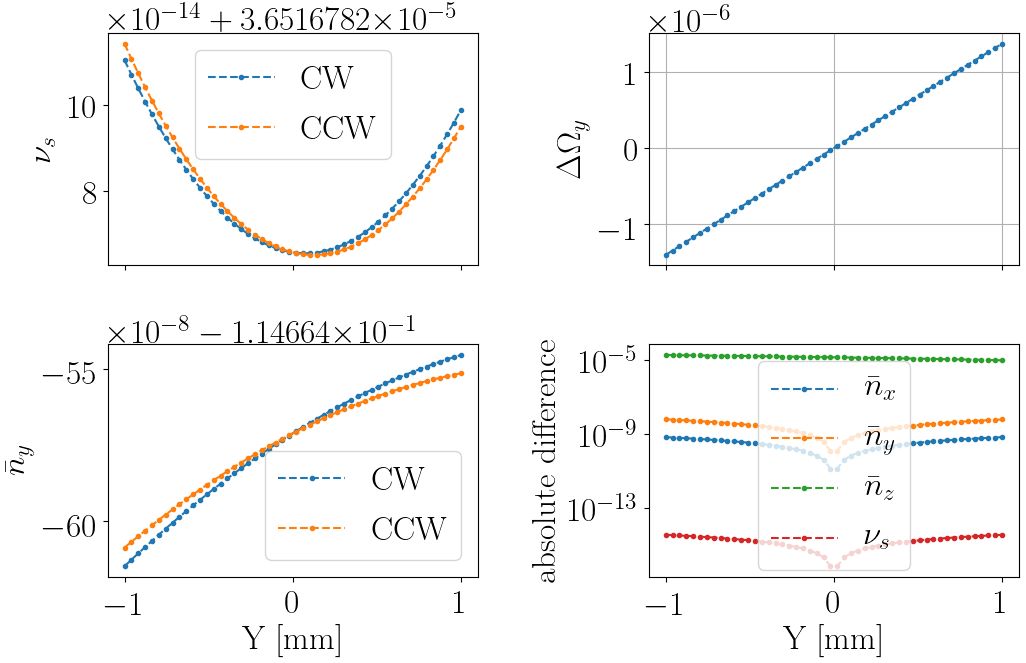
\includegraphics[width=\linewidth]{../img/IPAC19/GFF_stune_range_Y}
    \end{tikzfigure}
    \captionof{figure}{Spin tune and invariant spin axis dependencies on the particle vertical offset
      from the reference orbit for the CW and CCW moving beams}
    \begin{minipage}{.5\linewidth}
      \begin{tikzfigure}
        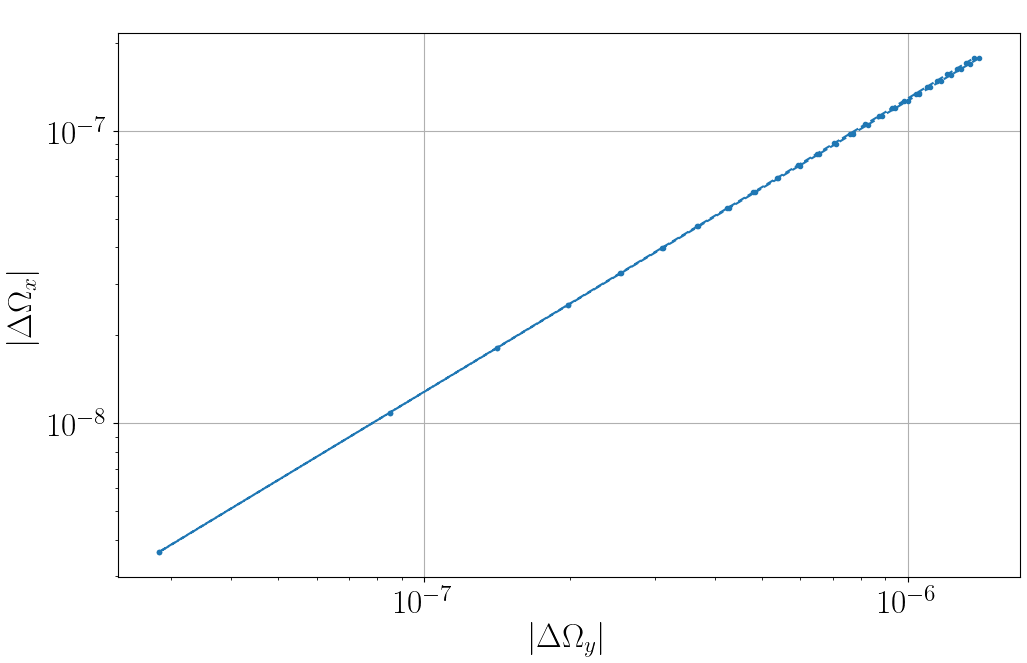
\includegraphics[width=\linewidth]{../img/IPAC19/GFF_omegas_range_Y}
      \end{tikzfigure}
      \captionof{figure}{Calibration plot in the vertical betatron motion case}
    \end{minipage}~~~~
    \begin{minipage}{.5\linewidth}
      \begin{tikzfigure}
        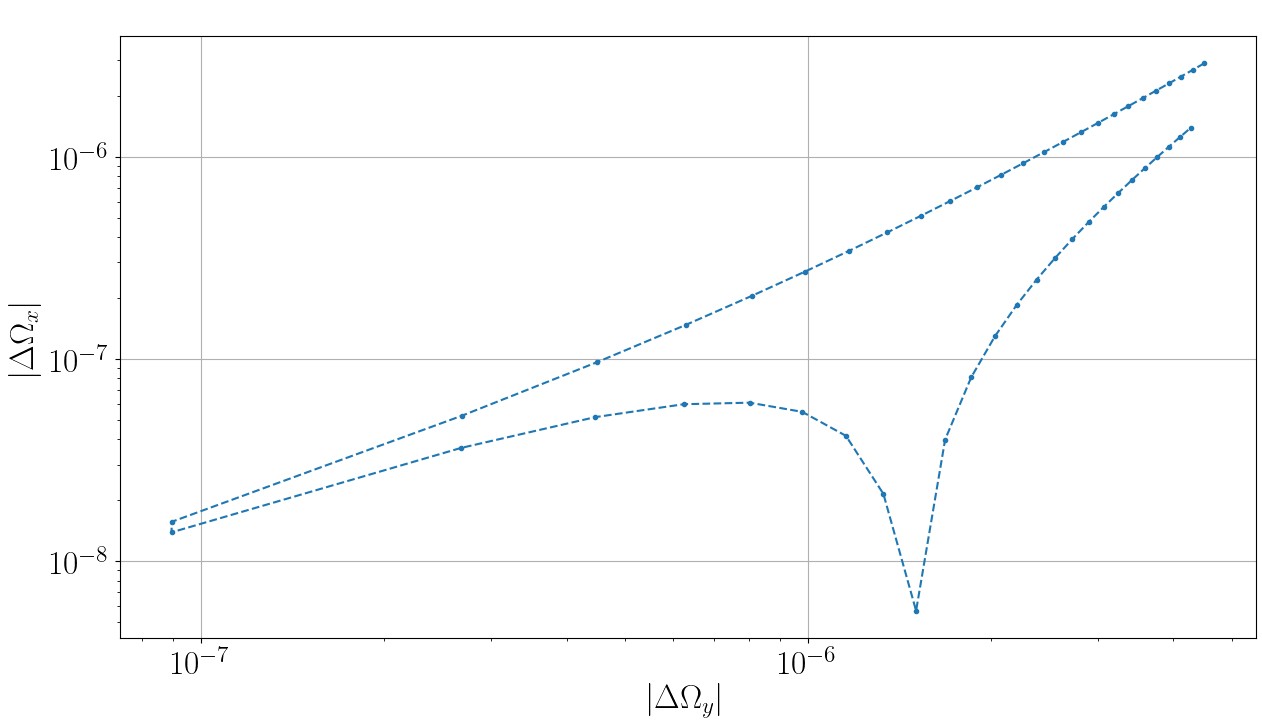
\includegraphics[width=\linewidth]{../img/IPAC19/GFF_omegas_range_X}
      \end{tikzfigure}
      \captionof{figure}{Calibration plot in the horizontal betatron motion case}
    \end{minipage}
    \begin{minipage}{.5\linewidth}
      \begin{tikzfigure}
        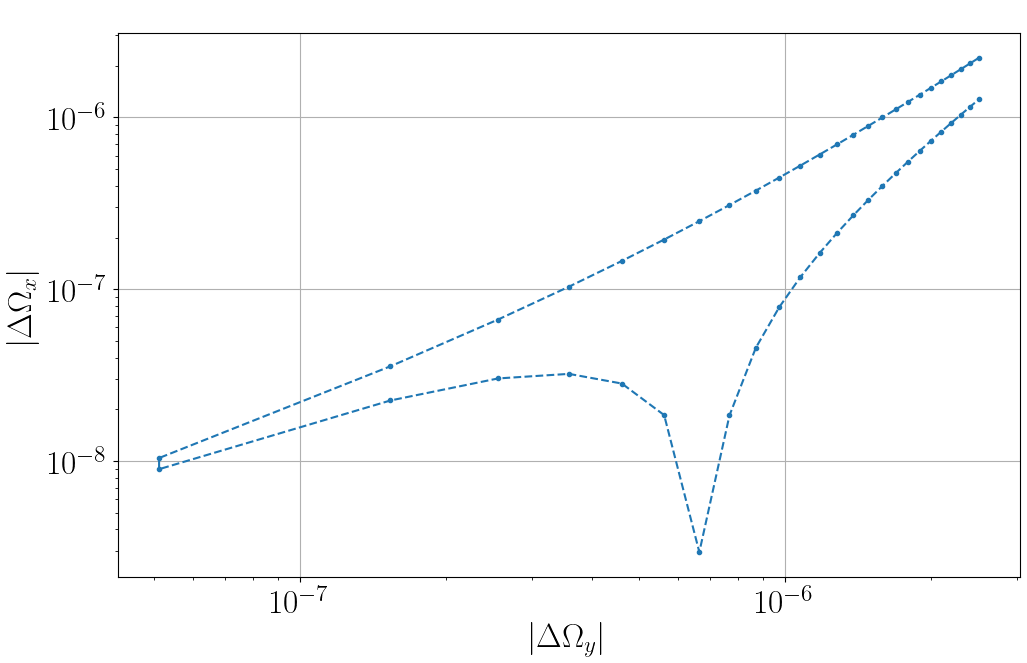
\includegraphics[width=\linewidth]{../img/IPAC19/GFF_omegas_range_D}
      \end{tikzfigure}
      \captionof{figure}{Calibration plot in the synchrotron motion case}
    \end{minipage}~~~~
    \begin{minipage}{.5\linewidth}
      \textbf{Conslusion}
      Equalization of the vertical plane MDM precession frequencies of counter-circulating
      beams by means of equalizing their horizontal plane precession frequencies is a viable technique.
    \end{minipage}
  }
  \column{.5}
  \block[bodyoffsety=2cm, titleoffsety=2cm]{PROBLEM STATEMENT}{
    \begin{itemize}
    \item The goal of flipping the direction of the guide field is to accurately reproduce the radial component
      of the MDM spin precession frequency induced by machine imperfection fields.
      
    \item A mere reproduction of the \emph{magnetic field strength} would not suffice,
      since the injection point of the beam's centroid, and hence its spin tune is subject to variation.

    \item Also, the accelerating structure might be asymmetrical, in terms of spin dynamics,
      with regard to reversal of the beam circulation direction.

    \item What needs to be reproduced, therefore, is not the field strength, but the effective Lorentz factor
      of the centroid.
    \end{itemize}
  }
  \block{EFFECTIVE L-FACTOR CALIBRATION}{
    \begin{itemize}
    \item Spin tune is an injective function of the effective Lorentz-factor $\g*$, which means
      $\W_y(\g*^1) = \W_y(\g*^2) \rightarrow \g*^1 = \g*^2$.
    \item Let $\Traj$ denote the set of all trajectories that a particle might follow in the accelerator.
    \item $\Traj$ is partitioned into equivalence classes according to the value of $\g*$.
    \item Since $\W_y(\g*)$ is injective,  $\exists!\g*^0$ at which $\W_y(\g*^0)=0$:
      $[\W_y=0] = [\g*^0]$.
    \item Once we ensure that the polarizations of both beams are frozen in the horizontal plane, their
      centroid's $\g*$ are equal.
    \end{itemize}
  }
  \block{SIMULATION}{
    \textbf{Need to show}
    \begin{enumerate}
    \item $[\g*^0]^{CW} = [\g*^0]^{CCW}$, that is $\W_y=0$ for the same set of trajectories in CW \& CCW.
    \item $\forall t_1,t_2\in [\g*^0]^{CCW}$: $\nu_s(t_1) = \nu_s(t_2)$, $\nbar(t_1) = \nbar(t_2)$, i.e.,
      the same sextupole fields reduce decohrerence in CCW as in CW.
    \end{enumerate}
    \textbf{How}
    \begin{enumerate}
    \item Compute $\nu_s(z)^{CW}$ and $\nu_s(z)^{CCW}$;
    \item Evaluate discrepancy $\epsilon(z) = \nu_s^{CW}(z) - \nu_s^{CCW}(z)$.
    \end{enumerate}
    \textbf{Analysis}\\
    If $\epsilon(z) \ll 1$ for a large range of $z\in \{x,y,\frac{\Delta p}{p}\}$, then
    \begin{itemize}
    \item sextupole decoherence suppression works for both beams without gradient value change;
    \item $\nu_s^{CW} \approx \nu_s^{CCW}$, and hence $\W_x^{MDM, CW} \approx \W_x^{MDM, CCW}$.
    \end{itemize}
  }
  \begingroup
  \renewcommand{\section}[2]{}%
  %\renewcommand{\chapter}[2]{}% for other classes
  \block{REFERENCES}{
    \begin{thebibliography}{9}
    \bibitem{BNL:Proton}
      V. Anastassopoulos et al., ``A Storage Ring Experiment to Detect a Proton Electric Dipole Moment.''
      Rev. Sci. Instrum., 87(11), 2016.
      \url{http://arxiv.org/abs/1502.04317}

    \bibitem{BNL:Deuteron2008}
      D. Anastassopoulos et al., ``AGS Proposal: Search for a permanent electric dipole moment of
      the deuteron nucleus at the $10^{-29}$ e$\cdot$cm level,'' BNL, 2008.
      
    \bibitem{Koop:SW}
      I. Koop,
      \textquotedblleft{Asymmetric Energy Colliding Ion Beams in the EDM Storage Ring}\textquotedblright,
      in \emph{Proc. 4th Int. Particle Accelerator Conf. (IPAC'13)}, Shanghai, China, May 2013, paper TUPWO040,
      pp. 1961--1963.
      \url{http://accelconf.web.cern.ch/accelconf/ipac2013/papers/tupwo040.pdf}

    %% \bibitem{Aksentev:IPAC19:GFF}
    %%   A. Aksentev, Y. Senichev, ``Simulation of the Guide Field Flipping Procedure for
    %%   the Frequency Domain Method,'' 
    %%   presented at the 10th International Particle Accelerator Conf. (IPAC'19), Melbourne, Australia,
    %%   May 2019, paper MOPTS010.


    \bibitem{Aksentev:IPAC19:Decoh}
      A. Aksentev, Y. Senichev, ``Spin decoherence in the Frequency Domain Method for the search of
      a particle EDM,''
      presented at the 10th International Particle Accelerator Conf. (IPAC'19), Melbourne, Australia,
      May. 2019, paper MOPTS012.

    \bibitem{Senichev:FDM}
      Y.~Senichev, A.~Aksentev, A.~Ivanov and E.~Valetov,
      %``Frequency domain method of the search for the deuteron electric dipole moment in a storage ring
      %with imperfections,''
      arXiv:1711.06512 [physics.acc-ph].
      %%CITATION = ARXIV:1711.06512;%%
      \url{https://arxiv.org/abs/1711.06512}

    \bibitem{Aksentev:FDM}
      A. Aksentev, Y. Senichev, E. Valetov, JEDI internal note \#4/2019.
    \end{thebibliography}
  }
  \endgroup
  

\end{columns}


\end{document}
